\subsection{Força Bruta}

Aquests algorismes són exactament el que sonen, mètodes senzills per resoldre un problema, provant totes les possibles possibilitats d'aquest fins a trobar la solució bona.

Per exemple, si tenim un cadenat de tres dígits entre 0 i 9 i ens oblidem de la contrasenya, com que no volem comprar un altre cadenat i no podem recordar cap dígit de la contrasenya, haurem d'utilitzar un mètode de força bruta per endevinar la contrasenya, és a dir, haurem de provar totes les possibilitats (0,0,0 / 0,0,1 / 0,0,2 / etc.), en el pitjor dels casos ens caldrien $10^3$ o 1000 intents, ja que tenim 3 dígits i per cada dígit hi ha 10 números diferents com a possibilitats, si tinguéssim un cadenat de 4 dígits, ara el nombre d'intents en el pitjor cas per trobar la contrasenya passaria a ser $10^4$ o 10000 intents .

Un exemple clàssic en informàtica és el problema del venedor ambulant (TSP). Suposem que un venedor ha de visitar 10 ciutats del país. Com es determina l'ordre en què s'han de visitar aquestes ciutats de manera que es minimitzi la distància total recorreguda?
La solució de força bruta és simplement calcular la distància total per a cada ruta possible i després seleccionar la més curta. Això no és especialment eficient perquè és possible eliminar moltes rutes possibles mitjançant algorismes inte\lgem igents, en canvi, la força bruta prova totes les opcions.

La complexitat temporal de la següent força bruta és $O(n \cdot m)$. Per tant, si cerquéssim una cadena de $n$ caràcters en una cadena de $m$ números mitjançant la força bruta, ens caldria $n \cdot m$ intents.

En la següent imatge veurem un algorisme de força bruta molt simple que endevina el codi d'un cadenat de 4 dígits. \newline

\begin{lstlisting}
void endivinarCodi(int contrasenya){
    for (int i = 0; i < 10000; i++){
        if (i == contrasenya){
        cout << "L'algorisme ha endevinat el teu codi!"<< endl;
        cout << "La contrasenya es: " << i << endl;
        }
    }
}

int main(){
    int contrasenya;
    cout << "Introdueix un codi, entre 0000 i 9999:" << endl;
    cin >> contrasenya;
    endivinarCodi(contrasenya);
}
\end{lstlisting}

\newpage

L'anterior codi el que fa és demanar un codi a l'usuari i després va provant dels números 0000 al 9999 i mira si coincideixen amb el codi donat.

És a\lgem ucinant la velocitat a la qual l'ordinador endevina el codi, és per això que és molt important tenir codis llargs i amb dígits diversos, puix que els $hackers$ utilitzen un l'algorisme de força bruta una mica modificat per endevinar els codis. \newline

\begin{center}
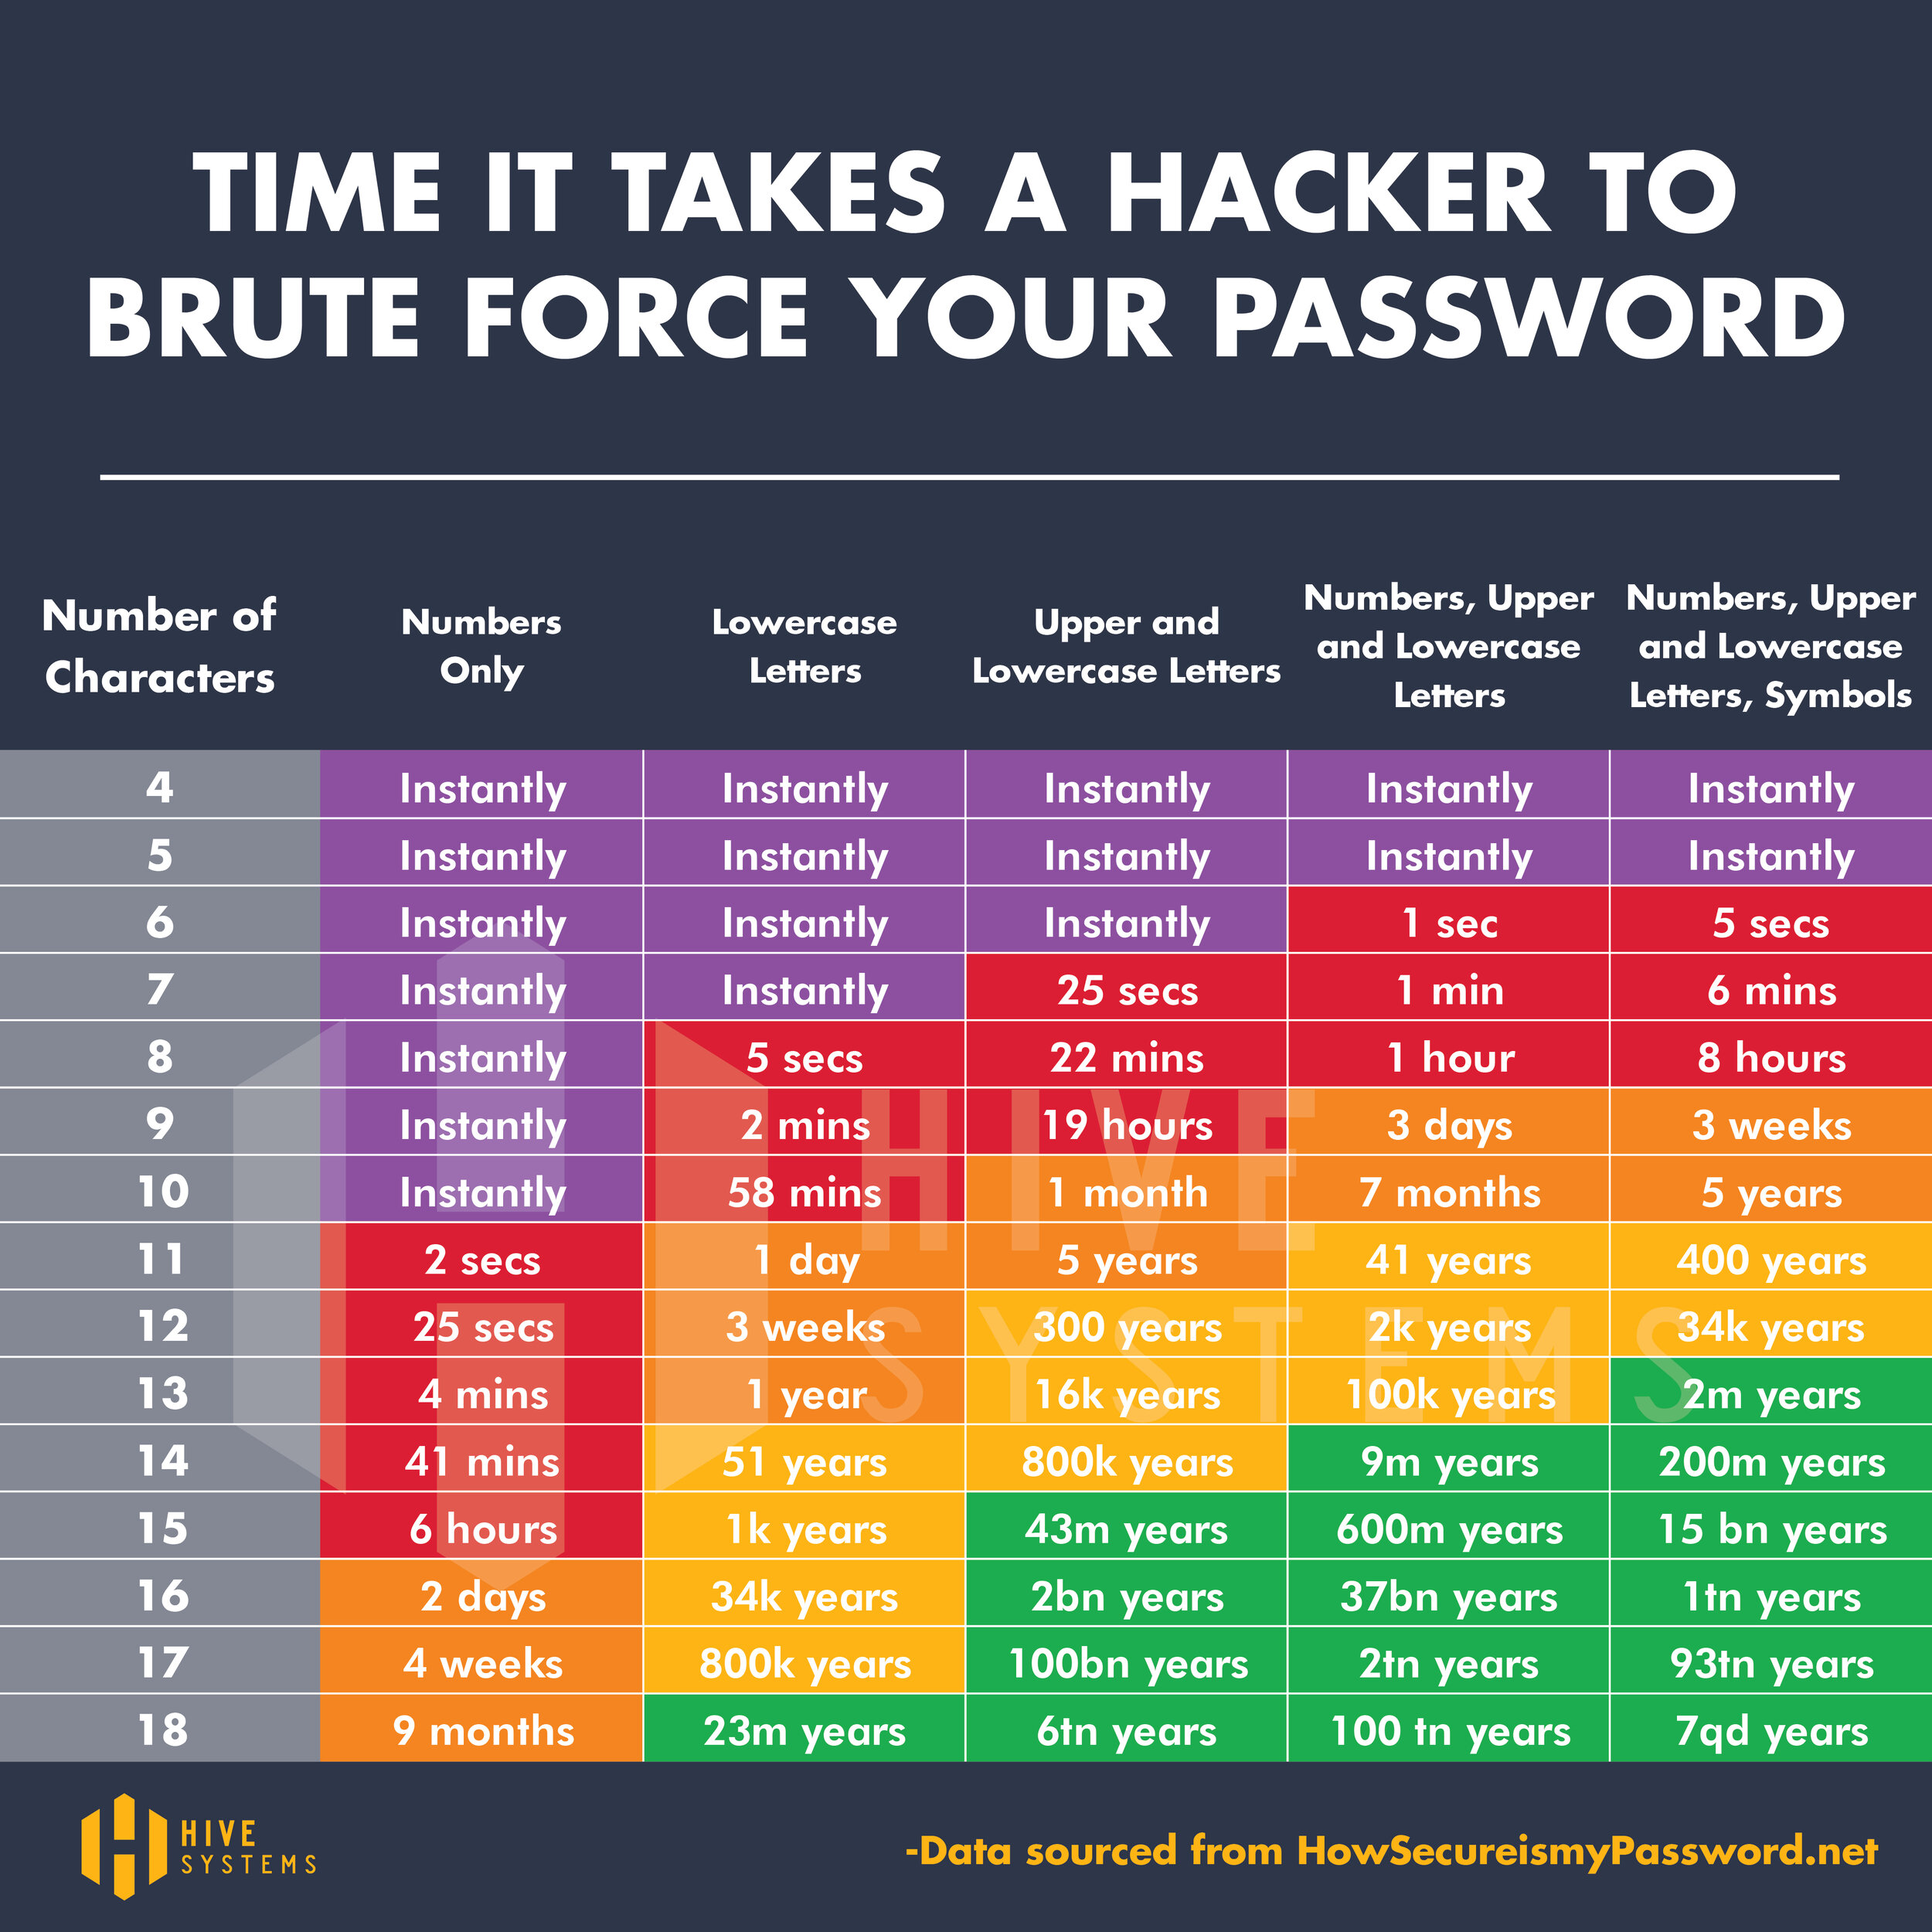
\includegraphics[width=.7 \textwidth]{time_hackers.jpg}

\caption{\emph{Figura 4: Temps en el qual els $hackers$ endevinen les contrasenyes mitjançant la força bruta.}}
\end{center}